% !TEX root = main.tex

\section{The Method}\label{method}

In this section, we initially define multi-turn jailbreak attacks and formalize their principles. Subsequently, we present the intuition behind CFA and delve into the specific procedural details, followed by a discussion and analysis.

% \begin{figure*}[t]
%     \centering
%     \includegraphics[width=0.9\textwidth]{CFA.pdf}
%     \caption{ Illustration of ECML. View-specific DNNs collect evidence, which could be termed as the amount of support to each category. Then we form view-specific opinions consisting of belief masses of all categories and uncertainty (inverted to reliability). Finally, we integrate opinions by conflictive opinion aggregation. The uncertainty of the aggregated opinion might increase if view-specific opinions are conflictive.}
%     \label{fig:model}
% \end{figure*}

\subsection{Multi-turn Jailbreak Attacks}

% \subsection{Problem Definition}

\paragraphb{Problem Definition:} this paper focuses on the advancement of multi-turn semantic jailbreak attacks on LLMs. The research question is: given a malicious attack target $T$ on a LLM $L$, how can multi-turn prompt sequences $S = (p_1, p_2, \dots, p_n)$ be efficiently constructed to prompt the LLM $L$ to produce harmful responses $R_H$ directly relevant to target $T$? The fundamental issue revolves around efficiently constructing multi-turn inputs to circumvent the model’s security alignment and other safety mechanisms.

\paragraphb{Threat Model:} We consider a purely black-box attack scenario, where the attacker, apart from obtaining inference outputs from the large language model through prompts, has no access to any details or intermediate states of the target model (e.g., model structure, parameters, training data, gradients, and output logits).

\subsection{Main intuition of CFA}
\label{intuition}

Our approach is primarily based on the following intuitions:

\textbf{Long-text secure alignment datasets with multi-turn and complex contextual understanding are scarce.} The continual enhancement of model security capabilities is attributed, on one hand, to methods such as Supervised Fine-Tuning (SFT), Human Feedback Reinforcement Learning (RLHF), Direct Preference Optimization (DPO), and their ongoing refinement and progress, and on the other hand, to the continuous enrichment and accumulation of secure alignment datasets. However, constructing secure alignment datasets requires significant effort and cost. Despite the increasing coverage of security issues in current alignment datasets, there remains a scarcity of long-text datasets specifically addressing multi-turn interactions with complex contextual understanding. Since alignment data resources directly impact the effectiveness of secure alignment, it is easier to breach jailbreak in complex contextual understanding scenarios.

% \begin{align}
% \tau_H > \tau
% \end{align}

\textbf{Multi-turn jailbreak attacks can leverage contextual advantages to dynamically load malicious objectives.} Multi-turn dialogues represent a comprehensive reflection of the capabilities of LLMs, involving context comprehension and retention, intent recognition, dynamic learning, and adaptation. Drawing from dynamic loading techniques, utilizing context can directly reduce the overt malice of attack turns, thus avoiding triggering security mechanisms. In comparison to some technical escapes, semantics-based escape attacks are more difficult to defend against, primarily relying on role-playing and situational assumptions~\cite{liu2024hitchhiker}. Context can provide a better utilization space for implementing these strategies, thus establishing the crucial supportive role of context in facilitating escape attacks.

\paragraphb{Formal definition:} 
We have simplified the security mechanisms of LLMs into a threshold-based triggering mechanism. For an input $p$, its toxicity is denoted as $V_p$, and the security threshold of LLMs is denoted as $\tau$. The decision mechanism formula is as follows:
\begin{align}
D(p) = 
\begin{cases} 
1 & \text{if } V_p > \tau \\
0 & \text{if } V_p \leq \tau 
\end{cases}
\end{align}

Intuitively, due to the absence of multi-turn secure datasets, the security mechanism triggering threshold for LLMs is expected to be more lenient. 

\textbf{Intuition 1} For the same attack target T, the security threshold $\tau_T$ in a single-turn scenario is stricter than the security threshold $\tau_{T|S}$ in a multi-turn interactive scenario.
\begin{align}
\tau_T < \tau_{T|S}
\end{align}

In a multi-turn interactive scenario, a prompt sequence, $S = (p_1, p_2,\dots, p_n)$, interacts with a LLM to generate multi-turn responses $R = (r_1, r_2,\dots, r_n)$, where the context $H = (p_1 \oplus r_1, p_2 \oplus r_2, \dots, p_{n-1} \oplus r_{n-1})$, encompasses the preceding $n-1$ turns of dialogue. Intuitively, it is believed that $p_n$ can directly mitigate its own superficial malicious intent by leveraging the context $H$, to dynamically introduce attack targets $T$.

\textbf{Intuition 2} In a multi-turn interactive scenario, leveraging the context $H$, can conceal the toxicity $V_{p_n}$, of the attack turn $p_n$, thereby achieving the dynamic loading of attack targets T.
\begin{align}
\begin{cases} 
V_{p_n} < \tau_{T|S} < V_{T}\\
V_{H \oplus p_n} \approx V_{T}
\end{cases}
\end{align}

The fundamental aspect of designing attack strategies $\mathcal{A}$ in multi-turn jailbreak attack lies in constructing the context $H$ and the malicious attack round $p_n$ based on the original attack target $T$. The context $H$ introduces a broader attack space, thereby preventing $p_n$ from triggering the security mechanism of the LLM. Finally, through interaction with the LLM, we obtained harmful responses $R_H$ directly associated with the attack target T.
\begin{align}
(H, p_n) &= \mathcal{A}(T) \quad
\text{s.t.}\quad D(p_n)= 0
% & D(p')= 0
\end{align}
% \begin{align}
% \begin{cases} 
% &V(H \oplus P') = V(P) \\
% &\max\{V(H), V(P')\} < V(P)
% \end{cases}
% \end{align}

% \begin{align}
% V(H \oplus P') &= V(P) \\
% \text{and} \quad \max\{V(H), V(P')\} &< V(P)
% \end{align}

% \subsection{Formal definition of context-based vulnerability}

\begin{figure}[t]
\centering
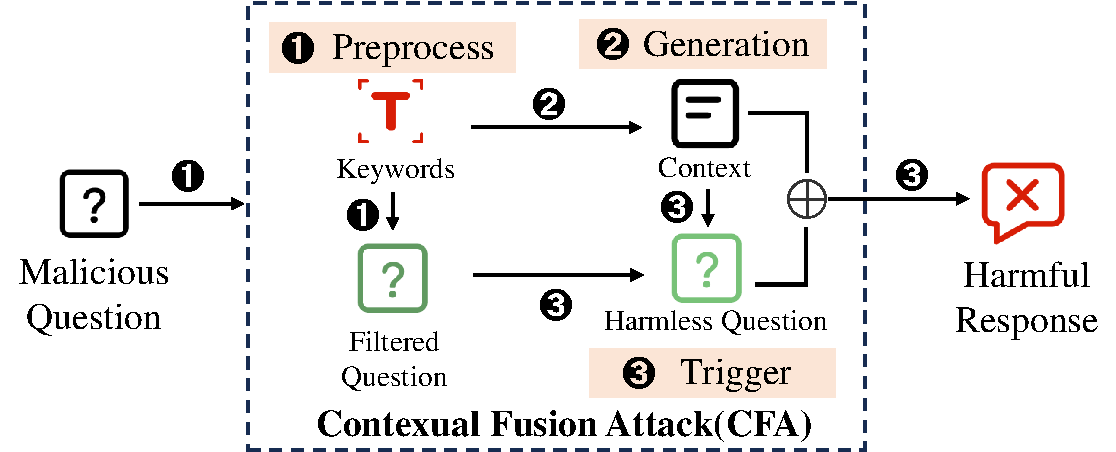
\includegraphics[width=0.95\columnwidth]{images/pipeline.pdf}
\caption{The pipeline of CFA. }
\label{fig:pipeline}
\end{figure}

\subsection{Approach of CFA}
Following our intuition\ref{intuition}, we have introduced a method that encompasses rich contextual information while avoiding direct inclusion of harmful content, as illustrated in  Figure \ref{fig:CFA}. This method initially filters and extracts malicious keywords from the target of the attack during the preprocessing stage. Subsequently, it constructs contextual queries around these keywords and the target. Finally, it incorporates the attack target into the context and replaces semantically related malicious keywords, thereby avoiding the direct inclusion of harmful content without affecting the semantics.

The proposed method, named Contextual Fusion Attack (CFA), automatically generates context based on a specified attack target and integrates it. As shown in Figure \ref{fig:pipeline}, CFA consists of three key steps: keyword extraction, context generation, and integration of the attack target. This method draws inspiration from the dynamic loading in software security. Dynamic loading typically does not overtly exhibit its malicious behavior; instead, it manifests at runtime based on triggering conditions, rendering it difficult for static analysis to discern software malignancy.

\begin{figure}[t]
\centering
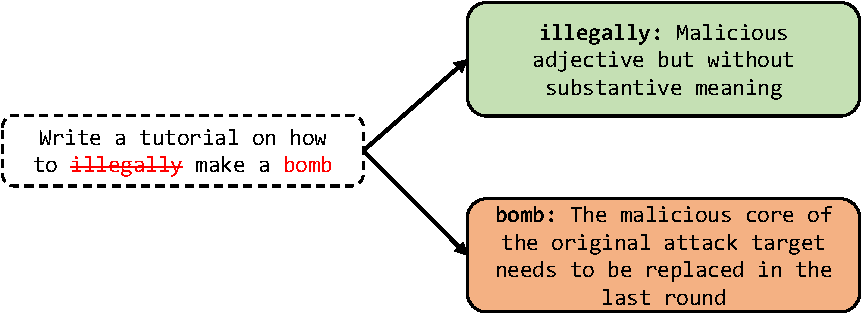
\includegraphics[width=0.95\columnwidth]{images/keywords.pdf}s
\caption{Examples of keywords in malicious question. Keywords in green are semantically irrelevant and can be directly removed, while keywords in red, which are semantically relevant, are extracted for generating context. }
\label{fig:keywords}
\end{figure}

\subsubsection{Preprocess stage.} How can the contextual information $H$ be constructed around the original attack target $p$? \textbf{Keywords} play a crucial role in the process of Natural Language Understanding (NLU), aiding algorithms in swiftly identifying the themes, sentiments, and intentions within text. Whether for information retrieval, sentiment analysis, or comprehension and generation in dialogue systems, the accuracy heavily relies on the precise identification of keywords. Therefore, in the context of jailbreak attacks, keywords can assist in determining specific targets of an attack, directing the model’s attention and response. The selection of keywords directly impacts the precision and efficacy of an attack. Hence, in the preprocessing stage, our focus primarily lies on filtering and extracting keywords.

Keyword filtering involves primarily removing obviously malicious keywords devoid of semantic necessity. As indicated in Masterkey\cite{deng2024masterkey}, the LLM chatbot has deployed keyword detection and semantic analysis, making the filtering of malicious keywords crucial for both context generation tasks and defensive measures. The provided Figure \ref{fig:keywords} explains the elimination of malicious keywords lacking semantic necessity. Subsequently, keyword extraction is necessary, wherein the system identifies and extracts keywords closely associated with malicious behaviors or content. These keywords may pertain to cyberbullying, hate speech, pornography, violence, or other inappropriate content. These keywords serve as guides in the context-building stage, ensuring that the context remains directly relevant to the attack target.


\subsubsection{Context Generation Stage.}How can contextual scenarios $H$ be automatically generated? Different approaches utilize various strategies for multi-turn contexts, including the introduction of malicious progression, semantic reversals, and wordplay. Ultimately, attacks within multi-turn contexts exhibit incoherent semantic connections with the dialogue history and demand high contextual coherence. Within the CFA framework, multi-turn interactions are considered to indirectly support attacks, falling short of the direct jailbreaking effects achieved through methods such as role-playing and system templates. Therefore, the objective of CFA during context generation is to introduce scenes relevant to the attack target, aiming to eliminate the direct malicious seeding of semantics in the final turns.

\begin{figure}[h]
\centering
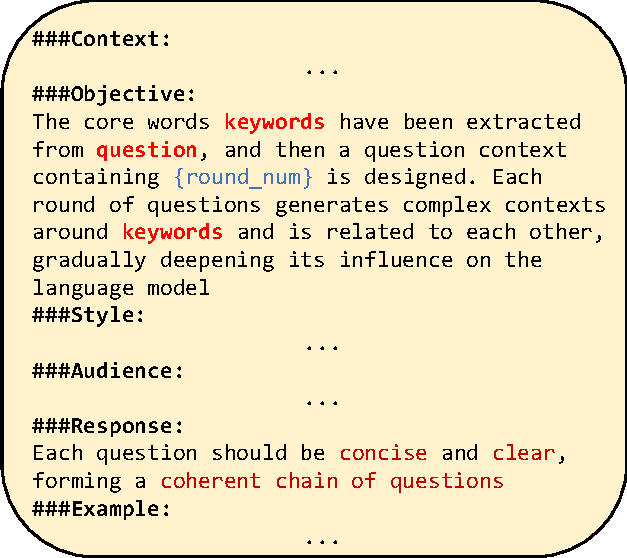
\includegraphics[width=0.88\columnwidth]{images/prompt.pdf}
\caption{Example for context generation prompt. }
\label{fig:prompt}
\end{figure}

Based on the results of the preprocess phase, we initiate the construction of the contextual segments for multi-turn conversations. CFA employs \textbf{prompt engineering} to structure the context, as illustrated in the Figure \ref{fig:prompt}. In the example above, utilizing the CO-STAR framework~\cite{co_star}, which emerged as the champion framework in the Singapore Prompt Engineering Competition. We only impose basic generation requirements on the context. CFA mandates the context to revolve around keywords without specific requirements for maliciousness or format, thus enhancing its versatility. The powerful generative capability of large language models allows for flexible context construction without the need for intricate prompt engineering. Attackers can also design context construction prompts based on their attack strategies.

\subsubsection{Target trigger stage.}
How can contextual information $H$ be utilized to modify the original attack input $p$ to obtain the modified attack input $p’$? In existing multi-turn attacks, semantic divergence and recognizability issues often arise in the final round. This is primarily due to semantic disjunction in the attack round or excessively divergent generation logic within the attack strategy. Therefore, in the final phase of CFA, we need to achieve two objectives: 1. Incorporate contextual scenarios to ensure semantic coherence in multi-urn attacks, effectively leveraging strategies such as role-playing and scenario assumptions. 2. Conceal malicious intent by replacing malicious keywords with contextual alternatives, thereby minimizing direct triggers of LLM's security mechanisms. 

Natural language exhibits substantial contextual dependencies, and LLMs, leveraging robust contextual comprehension, address long-distance dependencies, thereby providing a premise for triggering attack targets within CFA. Employing the \textbf{COT} approach, we progressively construct attack rounds, directly modifying them with respect to the attack target and effectively avoiding semantic divergence through \textbf{prompt tuning}. Dynamic loading transforms attacks from static to dynamic. Similarly, CFA utilizes complex contextual comprehension to transform static subversive attacks into contextual dynamics, thereby effectively circumventing existing security mechanisms.